\documentclass[12pt, a4paper]{article}
\usepackage{tikz}
\usepackage{graphics}
\usepackage{amsmath}


% Title Page
\title{Evolving Tower-Destroying Robots\\\normalsize An Exploration into Scaffolded Learning}
\author{Ryan Boldi}


\begin{document}
\maketitle
\tableofcontents
\newpage
\section{Goals}
We do not teach linear algebra to 6 year olds due to the fact that they do not have sufficient educational \emph{scaffolding} to grasp such a bizarre concept. My goal was to see whether or not this also applies to a robot evolving to do a certain task.\par 
The robot's task is to destroy a tower that starts a specific distance away from it:\par
\vspace{-10pt}
\begin{figure}[h]
	\label{goal}
\begin{center}
	\centering
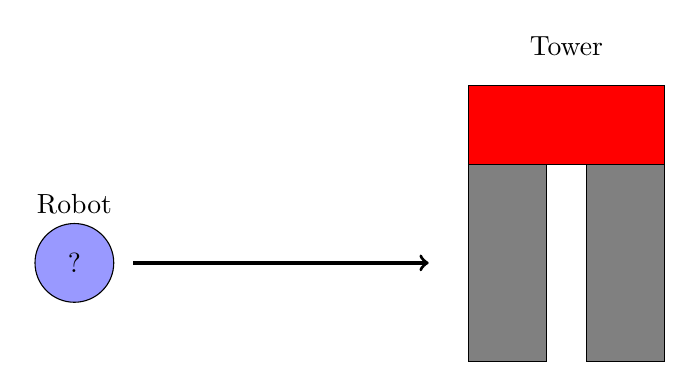
\begin{tikzpicture}
\filldraw[fill=blue!40!white](0,1.25) circle (5mm);
\node[] at (0,1.25) {?};
\node[] at (0,2) {Robot};
\draw [->, very thick] (0.75, 1.25) -- (4.5,1.25);
\filldraw[fill=gray] (5,0) rectangle (6,2.5);
\filldraw[fill=gray](6.5,0) rectangle (7.5,2.5);
\filldraw[fill=red] (5,2.5) rectangle (7.5,3.5);
\node[] at (6.25,4) {Tower};
\end{tikzpicture}
\caption{Diagram demonstrating the robot's task.}
\end{center}
\end{figure}
\vspace{-10pt}
To scaffold the learning of the robot, I planned to start the tower close to the robot, and slowly move it farther and farther away over the course of many generations. This will continue until the tower is at the goal distance from the robot. These are environmental changes that starts the robot with an easy task, waits for the task to be complete, then makes the task slightly harder. This process is repeated until the robot has mastered the most difficult goal task.\par
My goal was to experiment with this process, seeing whether or not it actually improved the speed of solution discovery, or quality of the solutions themselves.
\newpage

\section{Implementation}
\paragraph{Robot}
I started by creating the robot. It was based on a simple quadruped, but with 2 added arms to make destroying the tower easier. All of the limb relative sizes can be controlled and fined tuned in \emph{constants.py}.\par
\begin{figure}[h]
\includegraphics{robot.png}
\caption{The \emph{Tower-Destroyer} Robot. It has 6 sensors: one on the tip of each limb. It may move its legs and arms freely, each with 2 degrees of freedom. Each motor is controlled by the output layer of a fully connected neural network, which takes the sensor data as inputs. }
\end{figure}
\paragraph{Tower}
The Tower is created out of 3 similar cuboids, with the third balanced on top of the bottom two (see figure~\ref{goal}). The block colored in red is to be my `fall detector'. If this block comes into contact with the ground, we will count this tower as ``Fallen". If the tower has fallen over, the creature will receive a large fitness reward.
\paragraph{Fitness} To ensure that the reinforcement is not too sparse, I wanted to include an incentive to move towards the tower. After much deliberation, this is the fitness function I have included:
$$
\text{Fitness} = \begin{cases}
\text{distance from origin}_y & \text{if tower did not fall};\\
20 & \text{if tower fell.}\\
\end{cases}
$$

\noindent I believed that this would promote movement in the positive $y$ direction before the tower is in the robot's reach.

\paragraph{Scaffolding} To control whether or not we are going to scaffold the robot's learning, I added a new constant to the program that controls how many generations of \emph{pretraining} will occur. During pretraining, the tower's distance starts at low value, and incrementally gets larger as the robot performs better. When these pretraining generations are completed, the tower's distance will be set to the maximum (goal) distance, and the evolution continues until all of the total generations have completed. If pretraining is set to 300, and total generations is set to 600, we will pretrain the population for 300 generations, slowly incremementing the tower's distance whenever a robot successfully knocks over a tower. At 300 generations, no matter the current distance of the tower, we move it to it's maximum distance for the final 300 generations. If pretraining is set to 0, and total generations is set to 600, we will start the tower at its maximum distance, and train the population on that for 600 generation without moving the tower.
\newpage
\section{Results}
My results were extremely interesting and unforseen.
\begin{figure}[h]
\centering
\includegraphics{0-600-100-1500/0-600-100-1500.png}
\caption{Result after 0 generations of pretraining, 600 generations total, 100 creatures, and each creature was evaluated for 1500 timesteps.}
\end{figure}
\section{Reflection}

\end{document}          
